% Filename: p2_start_with_vim@latex_with_vim.tex
% This code is part of LaTeX with Vim.
% 
% Description: LaTeX with Vim is free book about Vim, LaTeX and Git.
% 
% Created: 29.03.12 11:31:41 PM
% Last Change: 30.03.12 12:02:00 AM
% 
% Author: Raniere Gaia Costa da Silva, r.gaia.cs@gmail.com
% Organization:  
% 
% Copyright (c) 2010, 2011, 2012, Raniere Gaia Costa da Silva. All rights 
% reserved.
% 
% This file is license under the terms of a Creative Commons Attribution 
% 3.0 Unported License, or (at your option) any later version. More details
% at <http://creativecommons.org/licenses/by/3.0/>.
\chapter{Primeiros comandos} \label{sch:vim:start}
\section{Movimentando o cursor e saltos}
No \textit{modo de comando} a movimentação do cursor pode ser realizada pelas setas direcionais ou pelas teclas \lcode{h}, \lcode{j}, \lcode{k} e \lcode{l} que correspondem, respectivamente, a esquerda, abaixo, encima e direita.

Já no \textit{modo de entrada} a movimentação só pode ser feita pelas setas direcionais.

\subsection{Caracteres}
Pode-se realizar saltos ao movimentar o cursor em uma mesma linha e para isso deve-se digitar quantos caracteres devem ser saltados e em seguida a direção a ser tomada. Por exemplo, comando \lcode{8l} salta $8$ caracteres a direita e \lcode{20h} $20$ caracteres a esquerda.

\subsection{Palavras}
O comando \lcode{w} leva o cursor para a próxima palavra e \lcode{W} para a próxima precedida por um espaço.

O comando \lcode{b} leva o cursor para a palavra anterior e \lcode{B} para a anterior precedida por um espaço.

Já o comando \lcode{e} leva o cursor para o fim da palavra e \lcode{E} para o fim da próxima palavra precedida por um espaço.

\subsection{Sentenças e Parágrafos}
O comando \lcode{)} leva o cursor para a próxima sentença e \lcode{\}} para o próximo parágrafo.

Já o comando \lcode{(} leva o cursor para a sentença anterior e \lcode{\{} para o parágrafo anterior.

\subsection{Linha}
O comando \lcode{0} promove o cursor para o início da linha e \$ para o final.

Já comando \lcode{Enter} leva o cursor para a linha seguinte e \lcode{-} para a linha anterior.

É importante saber a diferença entre os comandos \lcode{j} e \lcode{Enter}. O comando \lcode{j} leva o cursor para a próxima linha mantendo a mesma coluna enquanto o comando \lcode{Enter} para o início da próxima linha. A diferença entre os comandos \lcode{k} e \lcode{-} é semelhante ao apresentado pelos comandos \lcode{j} e \lcode{Enter}.

Para pular diretamente para a quinta linha do documento pode-se utilizar o comando \lcode{:$5$} e de maneira análoga para qualquer outra linha.

\subsection{Tela}
No \textit{modo de comando} pode-se posicionar cursor em relação a janela. Para isso deve-se utilizar os comandos \lcode{H}, primeira linha da janela, \lcode{M}, meio da janela,  e \lcode{L}, última linha da janela.

\section{Busca}
O comando \lcode{f} seguido de um caractere busa a primeira ocorrência do mesmo a direita da atual posição do cursor e \lcode{F} a próxima ocorrência a esquerda. Por exemplo, para ir a próxima ocorrência da letra \lcode{a} deve-se utilizar o comando \lcode{fa} e para a ocorrência anterior da letra b \lcode{Fb}.

O comando \lcode{;} repete a busca.

Já o comando \lcode{/} e \lcode{?} seguido por uma string e finalizado por \lcode{Enter} efetuam a busca pela primeira ocorrência da string após o cursor e antes do mesmo, respectivamente. No caso de os caracteres \lcode{/} e \lcode{?} aparecerem na string eles devem ser precedidos por \textbackslash.

Para repetir a busca pode-se utilizar o comando \lcode{n}. Já o comando \lcode{N} realiza a busca no sentido contrário.

Destaca-se que o comando \lcode{/} ou \lcode{?} leva o cursor para última linha da janela como ilustrado na Figura \ref{fig:vim_search_screen}.
\begin{figure}[h!]
    \centering
    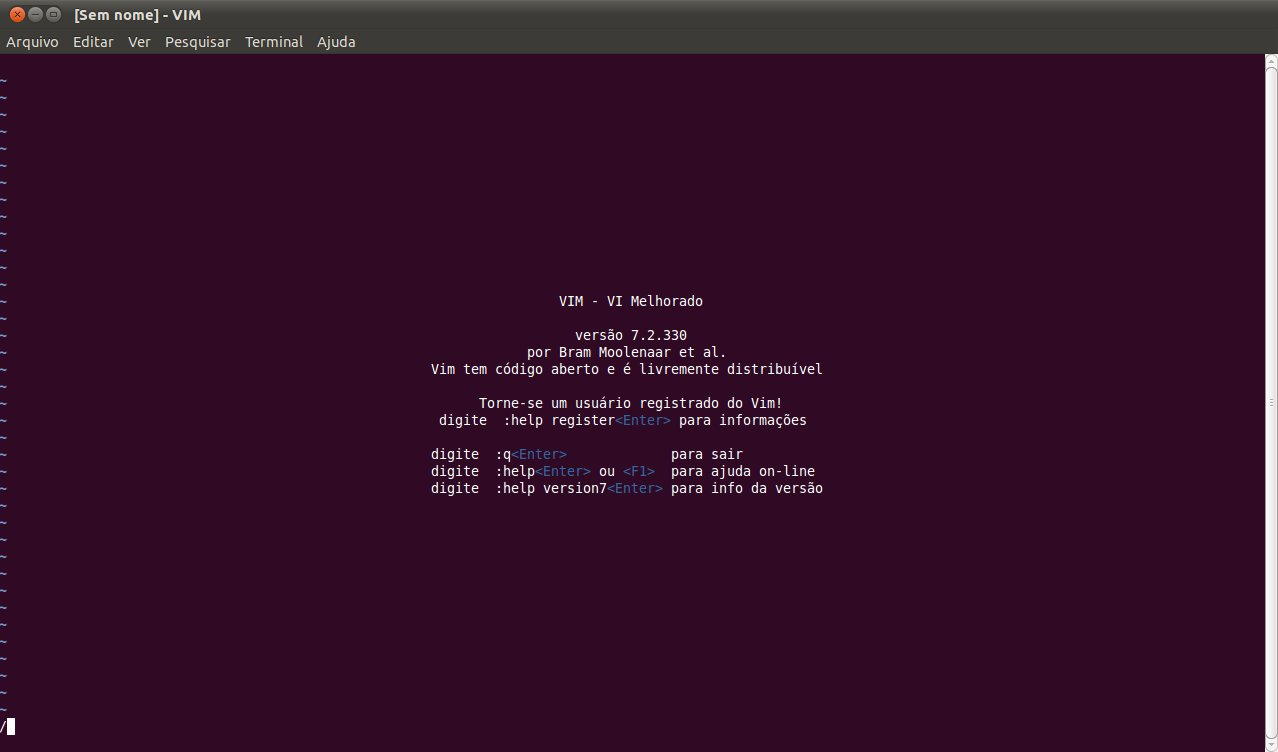
\includegraphics[height=6cm]{figures/vim_search_screen}
    \caption{Tela referente a busca.}
    \label{fig:vim_search_screen}
\end{figure}

Para localizar o par de um parênteses, colchetes ou chaves deve-se utilizar o comando \% quando o cursor estiver sobre um destes.

\section{Editando um texto}
\subsection{Linhas}
O comando \lcode{o} inicia uma nova linha abaixo da linha atual e iniciar o \textit{modo de edição} com o cursor posicionado na nova linha. Já \lcode{O} funciona de maneira semelhante ao \lcode{o} mas iniciando uma nova linha acima da linha atual.

O comando \lcode{J} junta a próxima linha a atual.

\subsection{Deletando}
Deve-se utilizar os comandos \lcode{x}, para apagar um único caractere, \lcode{dw}, para apagar uma palavra, e \lcode{dd}, para apagar uma linha.

O comando \lcode{X} apaga o primeiro caractere a esquerda do cursor.

É permitido utilizar um número antes do comando de forma que \lcode{6x} apaga 6 caracteres,  \lcode{3dw} apaga duas palavras e \lcode{2dd} apaga duas linhas.

O comando \lcode{d}\$ apaga do cursor ao fim da linha e \lcode{d}\textasciicircum apaga do cursor ao inicio da linha.

No \textit{modo de entrada} pode-se utilizar a tecla \lcode{Backspace} para apagar um único caractere.

O comando \lcode{Ctrl-w} suprimi o texto anterior ao cursor até o primeiro espaço.

\subsection{Mudando}
Para mudar uma palavra pode-se utilizar o comando \lcode{cw} que apaga a palavra e entra no \textit{modo de entrada}.

Os comandos \lcode{c}\$ e \lcode{c}\textasciicircum apagam, respectivamente até o fim da linha e até o começo da linha e passa ao \textit{modo de entrada}.

\subsection{Substituindo}
Para substituir uma única letra utiliza-se o comandos \lcode{r} seguido da nova letra. Para mais de uma letra utiliza-se \lcode{R} de modo que os novos caracteres substitui os antigos até que a tecla \lcode{Esc} seja pressionada. Logo após o comando \lcode{R} observa-se na última linha da janela a presençã do texto \lcode{- - SUBSTITUIÇÃO - -} como ilustrado na Figura \ref{fig:vim_replace_screen}.
\begin{figure}[h!]
    \centering
    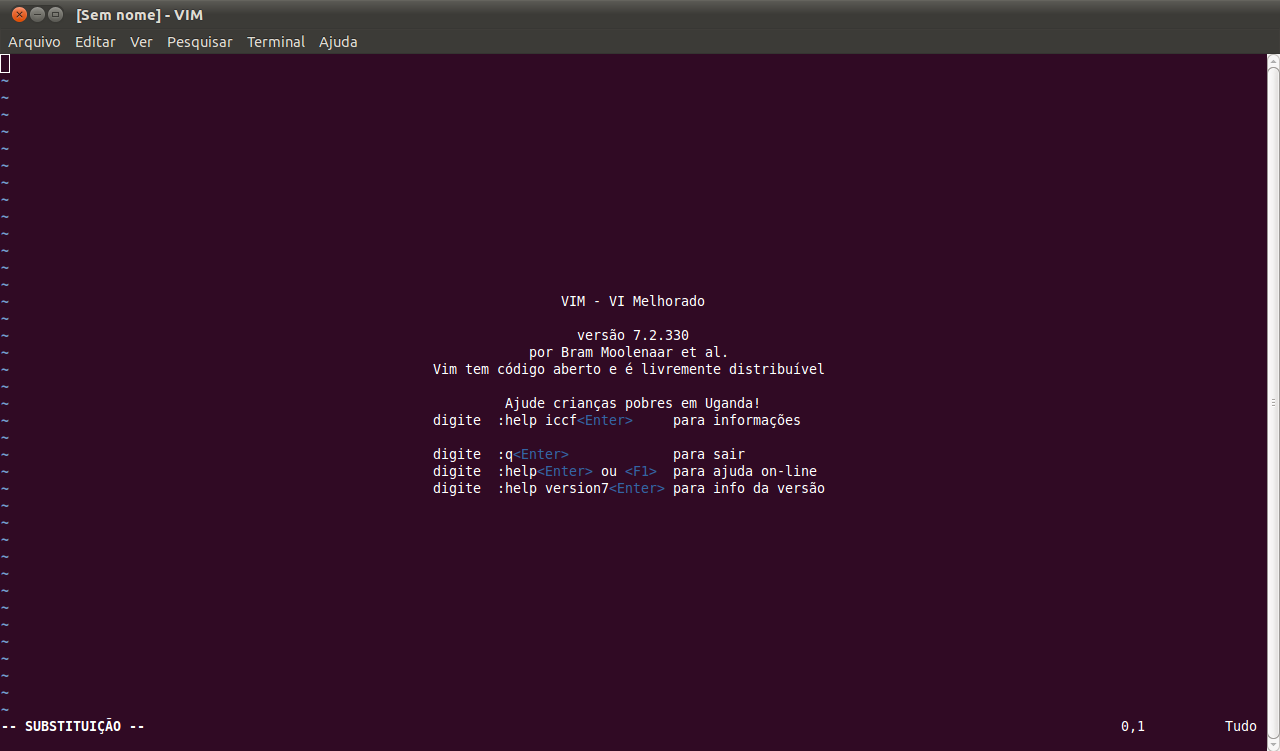
\includegraphics[height=6cm]{figures/vim_replace_screen}
    \caption{Tela após o comando \lcode{R}.}
    \label{fig:vim_replace_screen}
\end{figure}

\subsection{Trocando palavras}
Para trocar a primeira ocorrência de uma palavra por outra pode-se utilizar a sintaxe
\begin{code}
    :s/antiga/nova
\end{code}
onde \lcode{antiga} corresponde a palavra a ser substituida e \lcode{nova} a palavra que será utilizada para fazer a troca.

Para substituir todas as ocorrências de uma palavra em uma linha pode-se utilizar
\begin{code}
    :s/antiga/nova/g
\end{code}
e para todo o documento
\begin{code}
    :%s/antiga/nova/g
\end{code}

\subsection{Copiar, colar}
O comando \lcode{yy} ou \lcode{Y} copia a linha atual.

O comando \lcode{p} cola após o cursor e \lcode{P} antes a última informação copiada ou deletada.

\subsection{Inserindo arquivos}
Para inserir o conteudo de um arquivo no atual deve-se utilizar o comando
\begin{code}
    :r file
\end{code}
onde \lcode{file} é o nome do arquivo a ser inserido.

\section{Desfazer}
O comando \lcode{u} ou \lcode{:undo} desfaz a última alteração no texto. É permitido utilizar a tecla \lcode{u} mais de uma vez e com isso as alterações mais antigas são desfeitas. 

Ao errar em desfazer uma alteração pode-se utilizar as teclas \lcode{Ctrl}+\lcode{r} ou o comando \lcode{:redo}.
